%File: cogni_map_workshop.tex
\documentclass[letterpaper]{article}
\usepackage{aaai2026}
\usepackage{times}
\usepackage{helvet}
\usepackage{courier}
\usepackage[hyphens]{url}
\usepackage{graphicx}
\urlstyle{rm}
\def\UrlFont{\rm}
\usepackage{natbib}
\usepackage{caption}
\usepackage{amsmath}
\usepackage{amssymb}
\frenchspacing
\setlength{\pdfpagewidth}{8.5in}
\setlength{\pdfpageheight}{11in}

\pdfinfo{
/TemplateVersion (2026.1)
}

\setcounter{secnumdepth}{0}

\title{Cogni Map: Real-Time Detection of Cognitive Actions in Language Models Through Linear Probing}

\author{
    Ivan Chulo
}
\affiliations{
    Harvard University\\
    Cambridge, MA 02138 USA\\
    ichulo@g.harvard.edu
}

\begin{document}

\maketitle

\begin{abstract}
Understanding cognitive processes in large language models remains challenging, as we lack systematic tools to track internal reasoning patterns during text generation. To address this disconnect, we developed Cogni Map—a mechanistic interpretability tool leveraging linear probes to detect 45 cognitive actions spanning metacognitive, analytical, creative, and emotional categories. Binary one-vs-rest probes were trained on internal activations from 30 layers of Gemma-3-4B using 31,500 synthetic examples with augmented prompting for consistent extraction. Our approach achieved 0.78 average AUC-ROC across all cognitive actions, with layer 9 reaching peak performance (0.948 AUC). Distinct layer specialization emerged: mid-layers (5-24) capture high-level cognitive abstractions while early and late layers focus on surface features and next-token prediction. Application to therapy transcripts revealed therapist-dominant actions (\textit{perspective\_taking}, \textit{accepting}) versus client-dominant patterns (\textit{reconsidering}, \textit{self\_questioning}), aligning with person-centered therapy principles. Cogni Map bridges mechanistic interpretability and cognitive science, offering both quantitative probe analysis and qualitative exploration through an interactive terminal interface for understanding AI reasoning in diverse applications.
\end{abstract}

\section{Introduction}

Understanding the internal reasoning of large language models (LLMs) is crucial for ensuring their safety, interpretability, and alignment \cite{bereska2024mechanistic}. While previous studies have focused on profiling user attributes from conversations \cite{chen2024designing}, less attention has been given to identifying the \textit{cognitive actions} exhibited by the model during text generation.

This project introduces Cogni Map, a mechanistic interpretability tool designed to explore and annotate 45 cognitive actions spanning metacognitive, analytical, creative, and emotional categories. These actions, inspired by taxonomies from cognitive psychology, offer a detailed vocabulary for describing an AI's "thought processes," from \textit{pattern\_recognition} and \textit{hypothesis\_generation} to \textit{emotional\_reappraisal}. Cogni Map supports both quantitative analysis of cognitive patterns and qualitative exploration via an interactive TUI. The methodology is built upon linear probing techniques \cite{alain2016understanding} to extract representations of cognitive actions from transformer activations, enabling researchers to observe the cognitive functions that are active during generation.

\textbf{Contributions:} (1) A synthetic dataset of 31,500 examples with 700 per cognitive action; (2) Binary probes trained across 30 layers of Gemma-3-4B achieving 0.78 average AUC-ROC with layer specialization; (3) A toolkit for quantitative and qualitative analysis; (4) Practical application to therapy transcript analysis.

\section{Methodology}

\textbf{Cognitive Action Taxonomy.} A taxonomy of 45 cognitive actions was defined, organized into four categories: \textit{Metacognitive} (13 actions, e.g., \textit{reconsidering}, \textit{updating\_beliefs}), \textit{Analytical} (12 actions, e.g., \textit{analyzing}, \textit{evaluating}), \textit{Creative} (6 actions, e.g., \textit{divergent\_thinking}, \textit{reframing}), and \textit{Emotional} (14 actions, e.g., \textit{emotional\_reappraisal}).

\textbf{Activation Capture and Probing.} Following established probing methodologies \cite{alain2016understanding,chen2024designing}, activations were extracted from 30 of the 35 layers of Gemma-3-4B using nnsight. During both activation capture and inference, inputs were augmented with task-specific suffixes ("\textbackslash n\textbackslash nThe cognitive action being demonstrated here is" for cognitive probes; "\textbackslash n\textbackslash nThe sentiment of this section is" for sentiment probes) to ensure consistent extraction from the final token representation. A \textbf{one-vs-rest} strategy was used to train 45 independent binary linear probes, which allows for per-action interpretability and the flexibility to mix optimal layers for each action during inference. Training was performed with an AdamW optimizer, cosine annealing scheduler, and early stopping, using an AUC-ROC metric to handle the severe class imbalance.

\textbf{Data Generation.} The training dataset consists of 31,500 synthetic examples generated using Gemma 3 4b. This includes 700 examples for each of the 45 cognitive actions and 1,800 examples for sentiment analysis.

\section{Results}

\textbf{Probe Performance.} The binary probes demonstrated strong performance, achieving an average AUC-ROC of 0.78 and an average F1 score of 0.68 across all 45 cognitive actions. Top-performing probes included \textit{suspending\_judgment} (0.988 AUC) and \textit{counterfactual\_reasoning} (0.984 AUC), while more challenging actions included \textit{emotion\_responding} (0.778 AUC). These results confirm that cognitive actions have linearly separable representations within Gemma-3-4B's activation space \cite{alain2016understanding}.

\textbf{Layer Specialization.} A distinct pattern of layer specialization was observed across the 30 analyzed layers. Layer 9 yielded the best average performance (AUC-ROC: 0.9481), with a strong performance envelope across layers 5-24. Performance degraded in the earliest and latest layers, suggesting that early layers focus on surface-level features, mid-layers capture high-level cognitive abstractions, and late layers optimize for next-token prediction, potentially overwriting these representations. Notably, different cognitive actions peaked at different layers—for instance, \textit{divergent\_thinking} was best detected at layer 22, whereas \textit{pattern\_recognition} peaked at layer 9.

\textbf{Application: Therapy Transcript Analysis.} Cogni Map was applied to analyze a therapy session transcript, comparing the cognitive actions of the therapist and the client. The analysis revealed that therapist-dominant actions included \textit{perspective\_taking}, \textit{accepting}, and \textit{noticing}. In contrast, client-dominant actions were \textit{reconsidering}, \textit{emotion\_receiving}, and \textit{self\_questioning}. These findings align with the principles of person-centered therapy \cite{rogers1951client}, where the therapist fosters an environment for the client's self-exploration.

\section{Discussion and Future Work}

Cogni Map builds upon prior work in interpretability \cite{alain2016understanding,chen2024designing} but shifts the focus from modeling external users to tracking the internal cognitive processes of the model itself. While Chen et al. demonstrated probing for user demographics, we track cognitive actions in model-generated content—a complementary approach to representation engineering work \cite{zou2023representation}.

\textbf{Limitations} of this study include the reliance on synthetic data, the focus on a single model (Gemma-3-4B) and the assumption of independence between cognitive actions.

\textbf{Future directions} include extending the tool to larger models, training on human-annotated data, and exploring applications in AI safety, ToM in LLMs and AI alignment.

\textbf{Broader Impact:} This tool offers a means to explore AI reasoning patterns, which could help identify flawed logic, understand student thought processes in educational settings, and build more interpretable AI systems. The combination of quantitative probes and a qualitative TUI supports a wide range of use cases.

\section{Conclusion}

Cogni Map is a practical tool for exploring and annotating 45 cognitive actions in language models. By using linear probes on the internal activations of Gemma-3-4B, this work successfully identified and analyzed these actions, revealing specialized layer-dependent representations. The toolkit, which supports both quantitative and qualitative analysis, has demonstrated its utility in a real-world application, bridging the gap between mechanistic interpretability and cognitive science. The full source code, trained probes, and datasets are available on GitHub.

\bibliography{cogni_map_workshop}

\clearpage
\appendix

\section{Additional Visualizations}

\begin{figure*}[t]
\centering
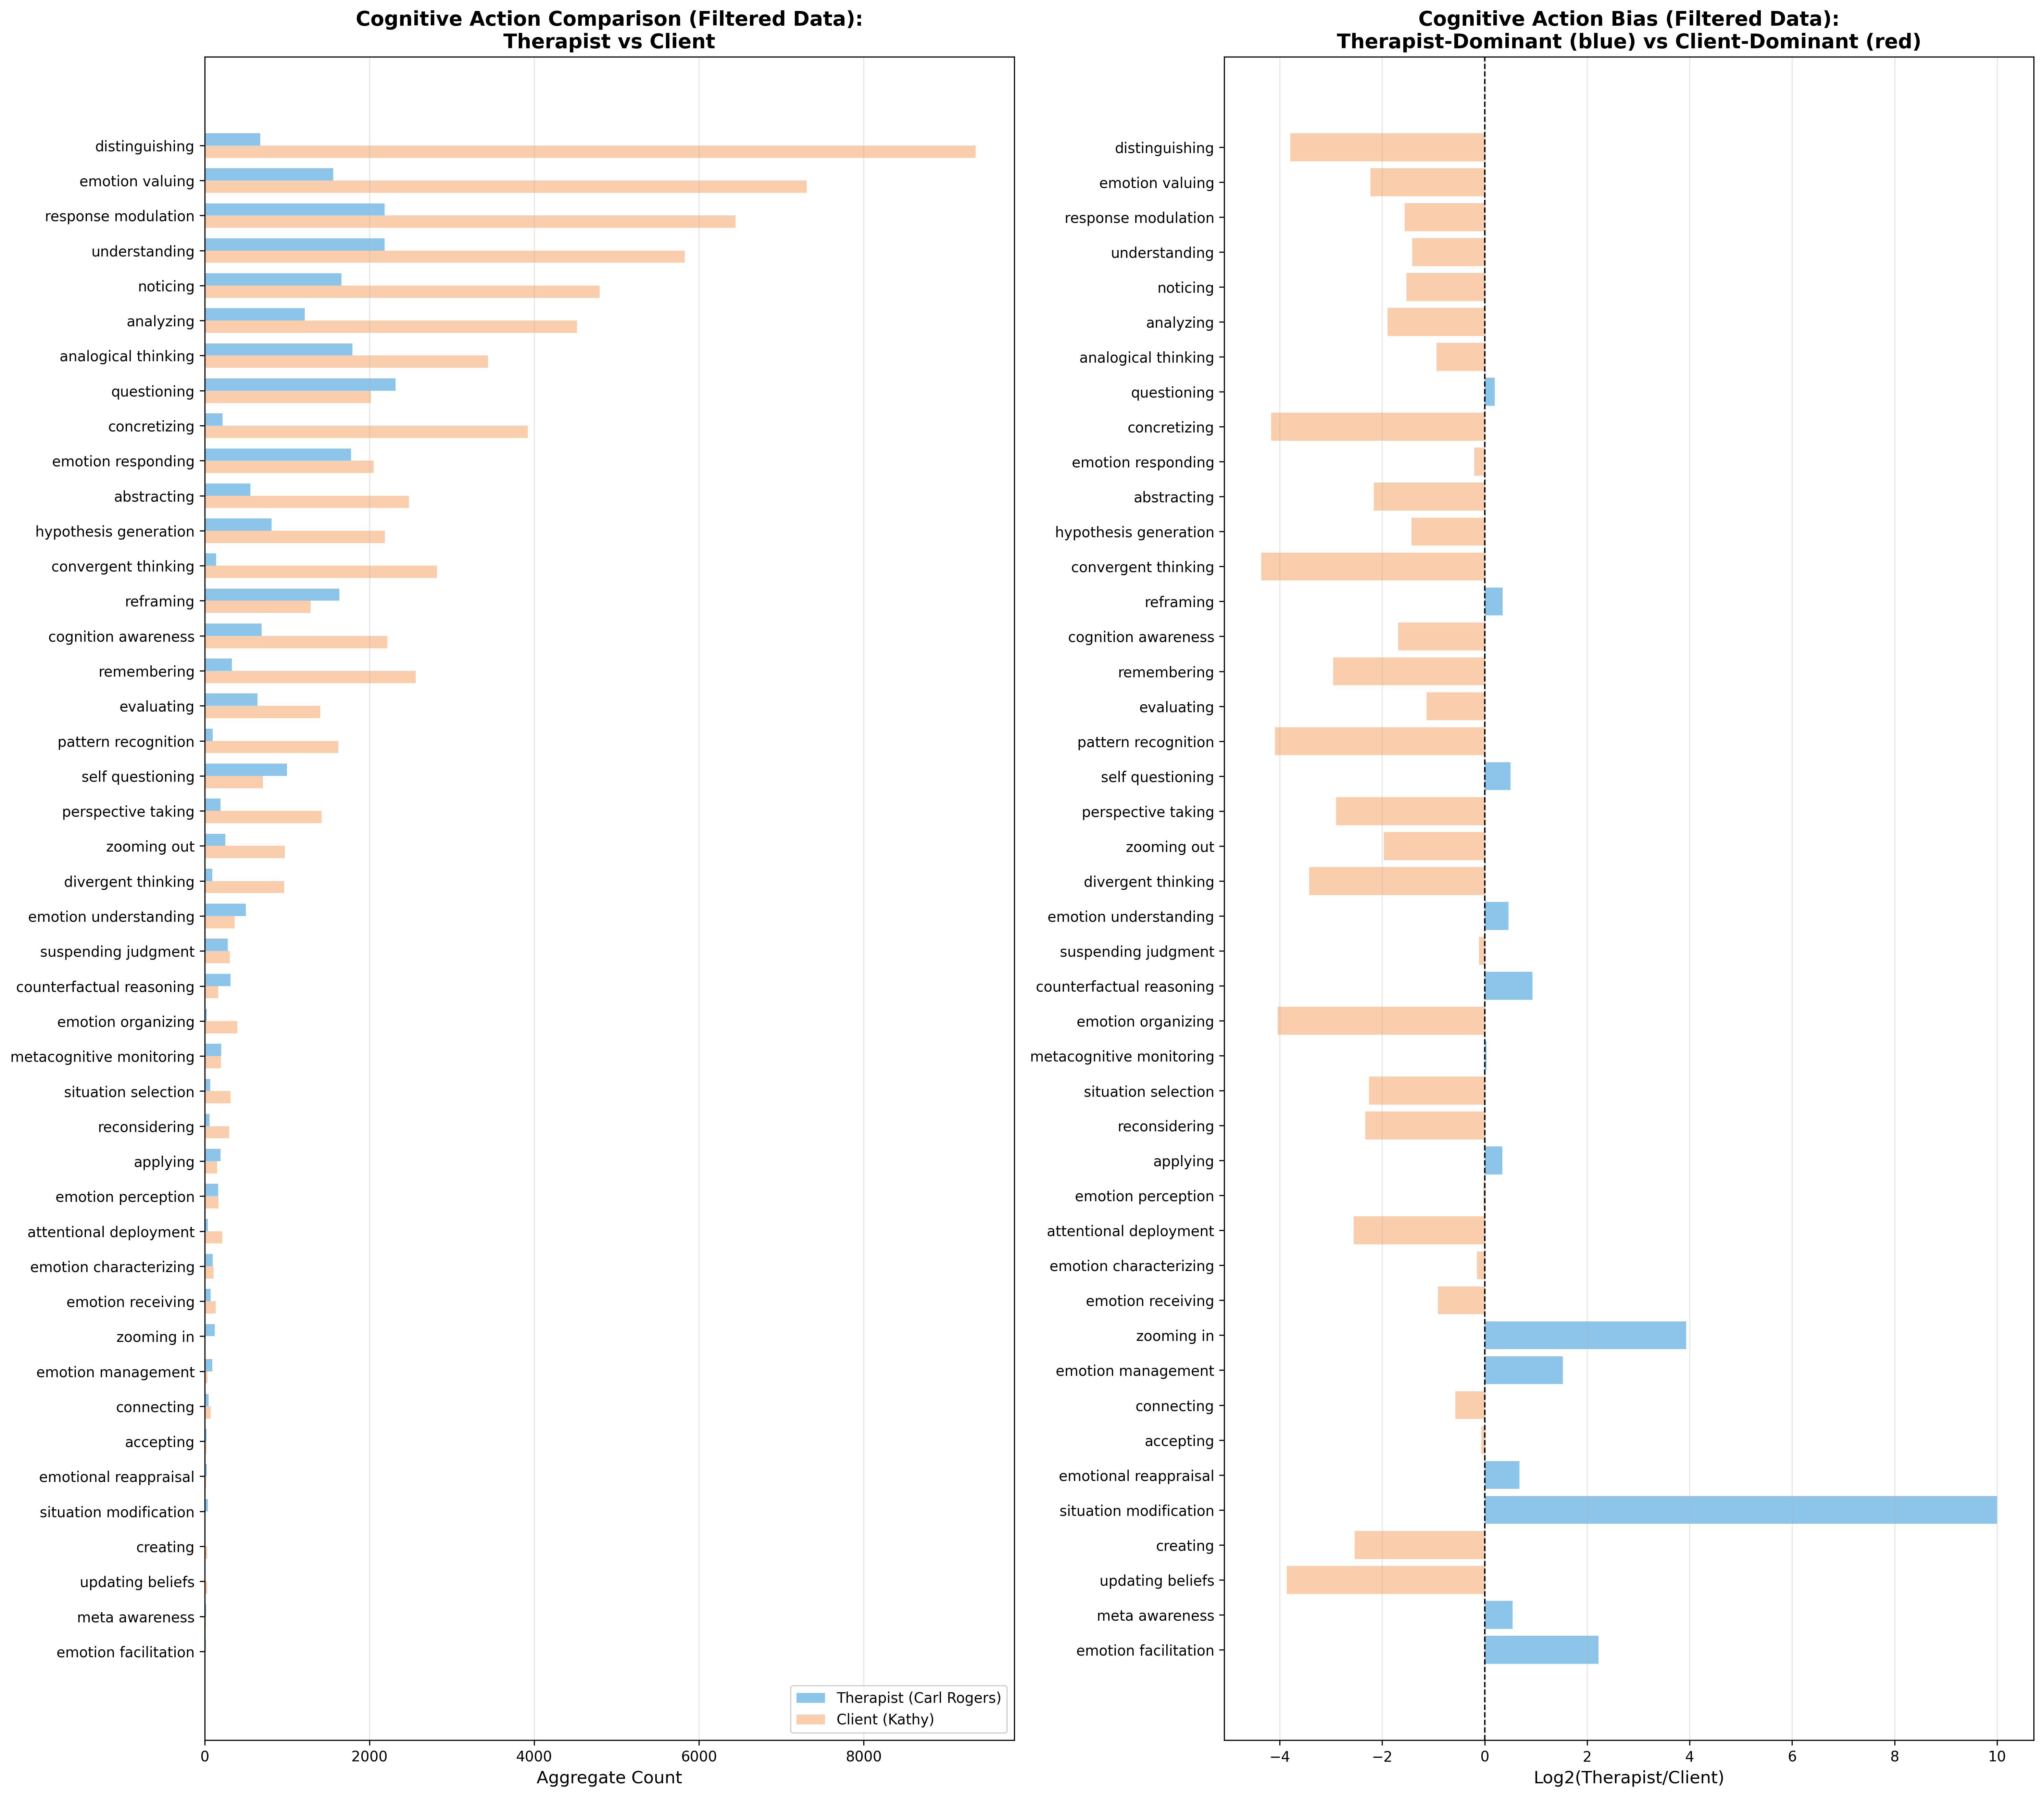
\includegraphics[width=\textwidth]{../Keep_viz/rogers_kathy_comparison.png}
\caption{Therapy session analysis comparing cognitive action patterns between therapist (Carl Rogers) and client (Kathy). Left panel shows aggregate counts of cognitive actions for both participants across filtered data. Right panel displays cognitive action bias as log2 ratio, highlighting therapist-dominant actions (blue) such as \textit{situation\_modification}, \textit{emotional\_reappraisal}, and \textit{emotion\_facilitation}, versus client-dominant actions (red) including \textit{zooming\_in}, \textit{self\_questioning}, and \textit{applying}. These patterns align with person-centered therapy principles.}
\label{fig:therapy_comparison}
\end{figure*}

\begin{figure*}[t]
\centering
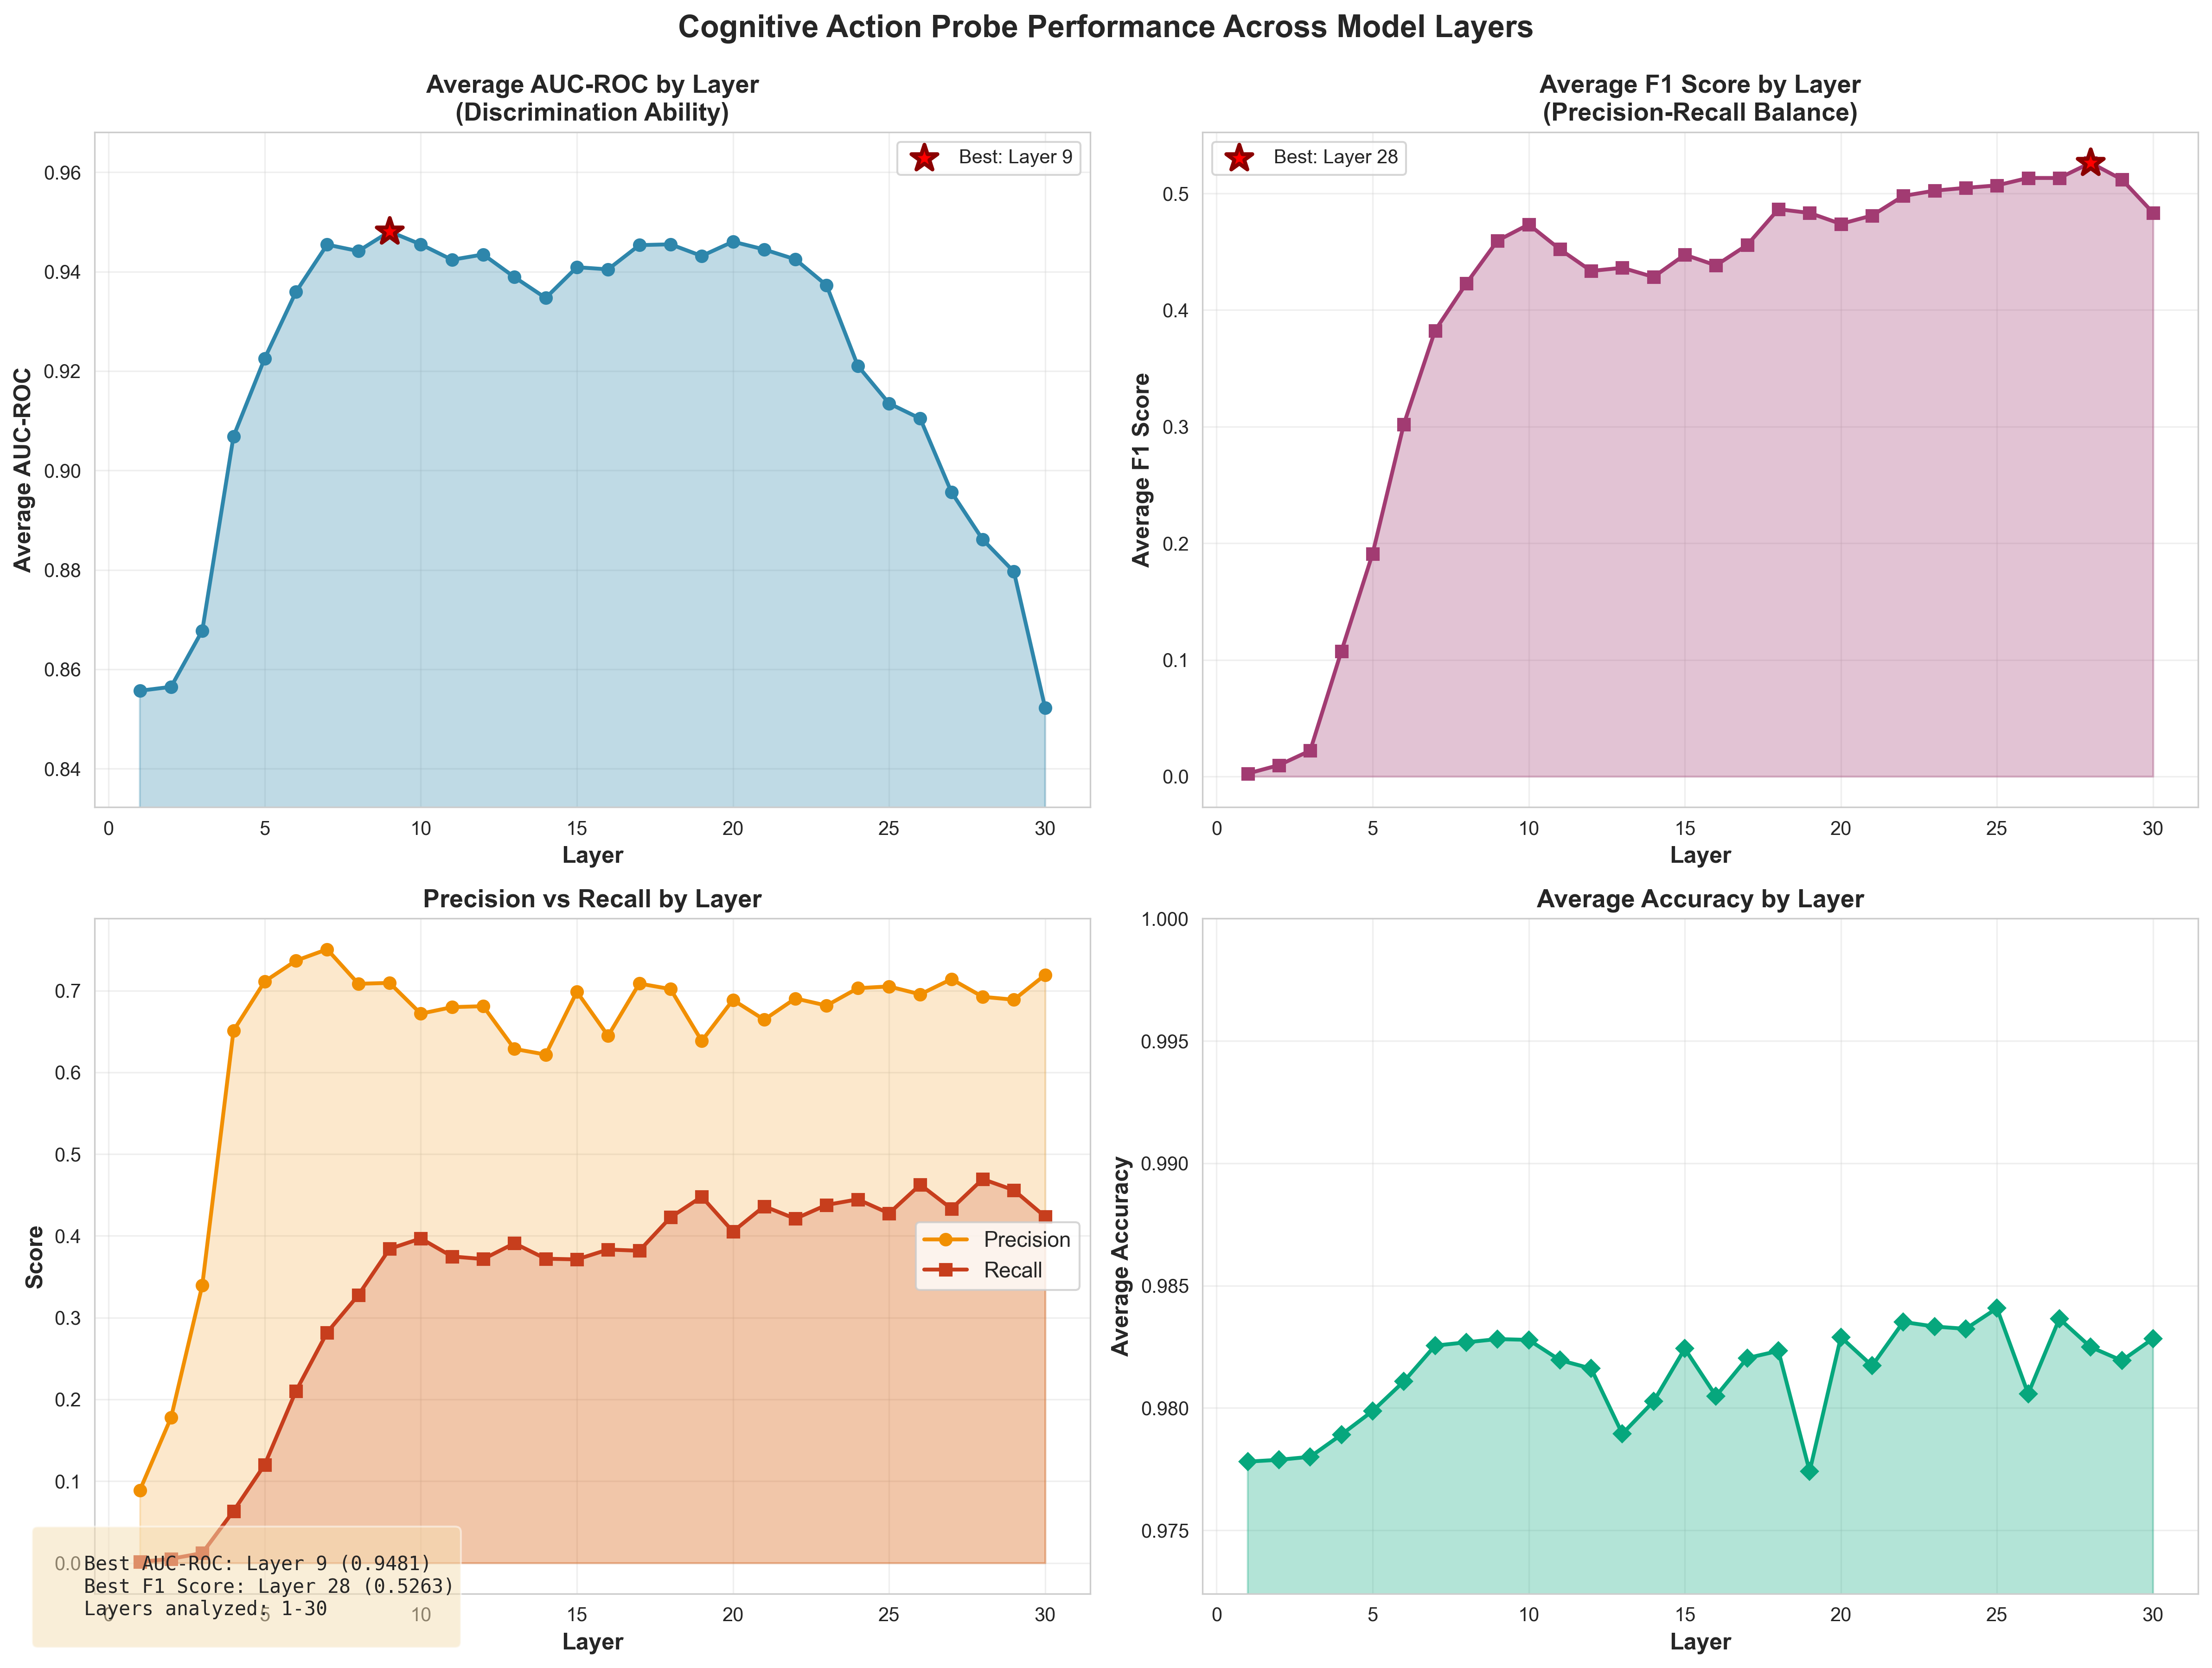
\includegraphics[width=\textwidth]{../data/cognitive_probe_performance_by_layer.png}
\caption{Cognitive action probe performance across all 30 layers of Gemma-3-4B. The visualization shows average AUC-ROC scores for each layer, with Layer 9 achieving peak performance (0.948 AUC-ROC). Strong performance is maintained across mid-layers (5-24), while early and late layers show degraded performance. This pattern suggests that early layers focus on surface-level features, mid-layers capture high-level cognitive abstractions, and late layers optimize for next-token prediction, potentially overwriting intermediate representations.}
\label{fig:layer_performance}
\end{figure*}

\begin{figure*}[t]
\centering
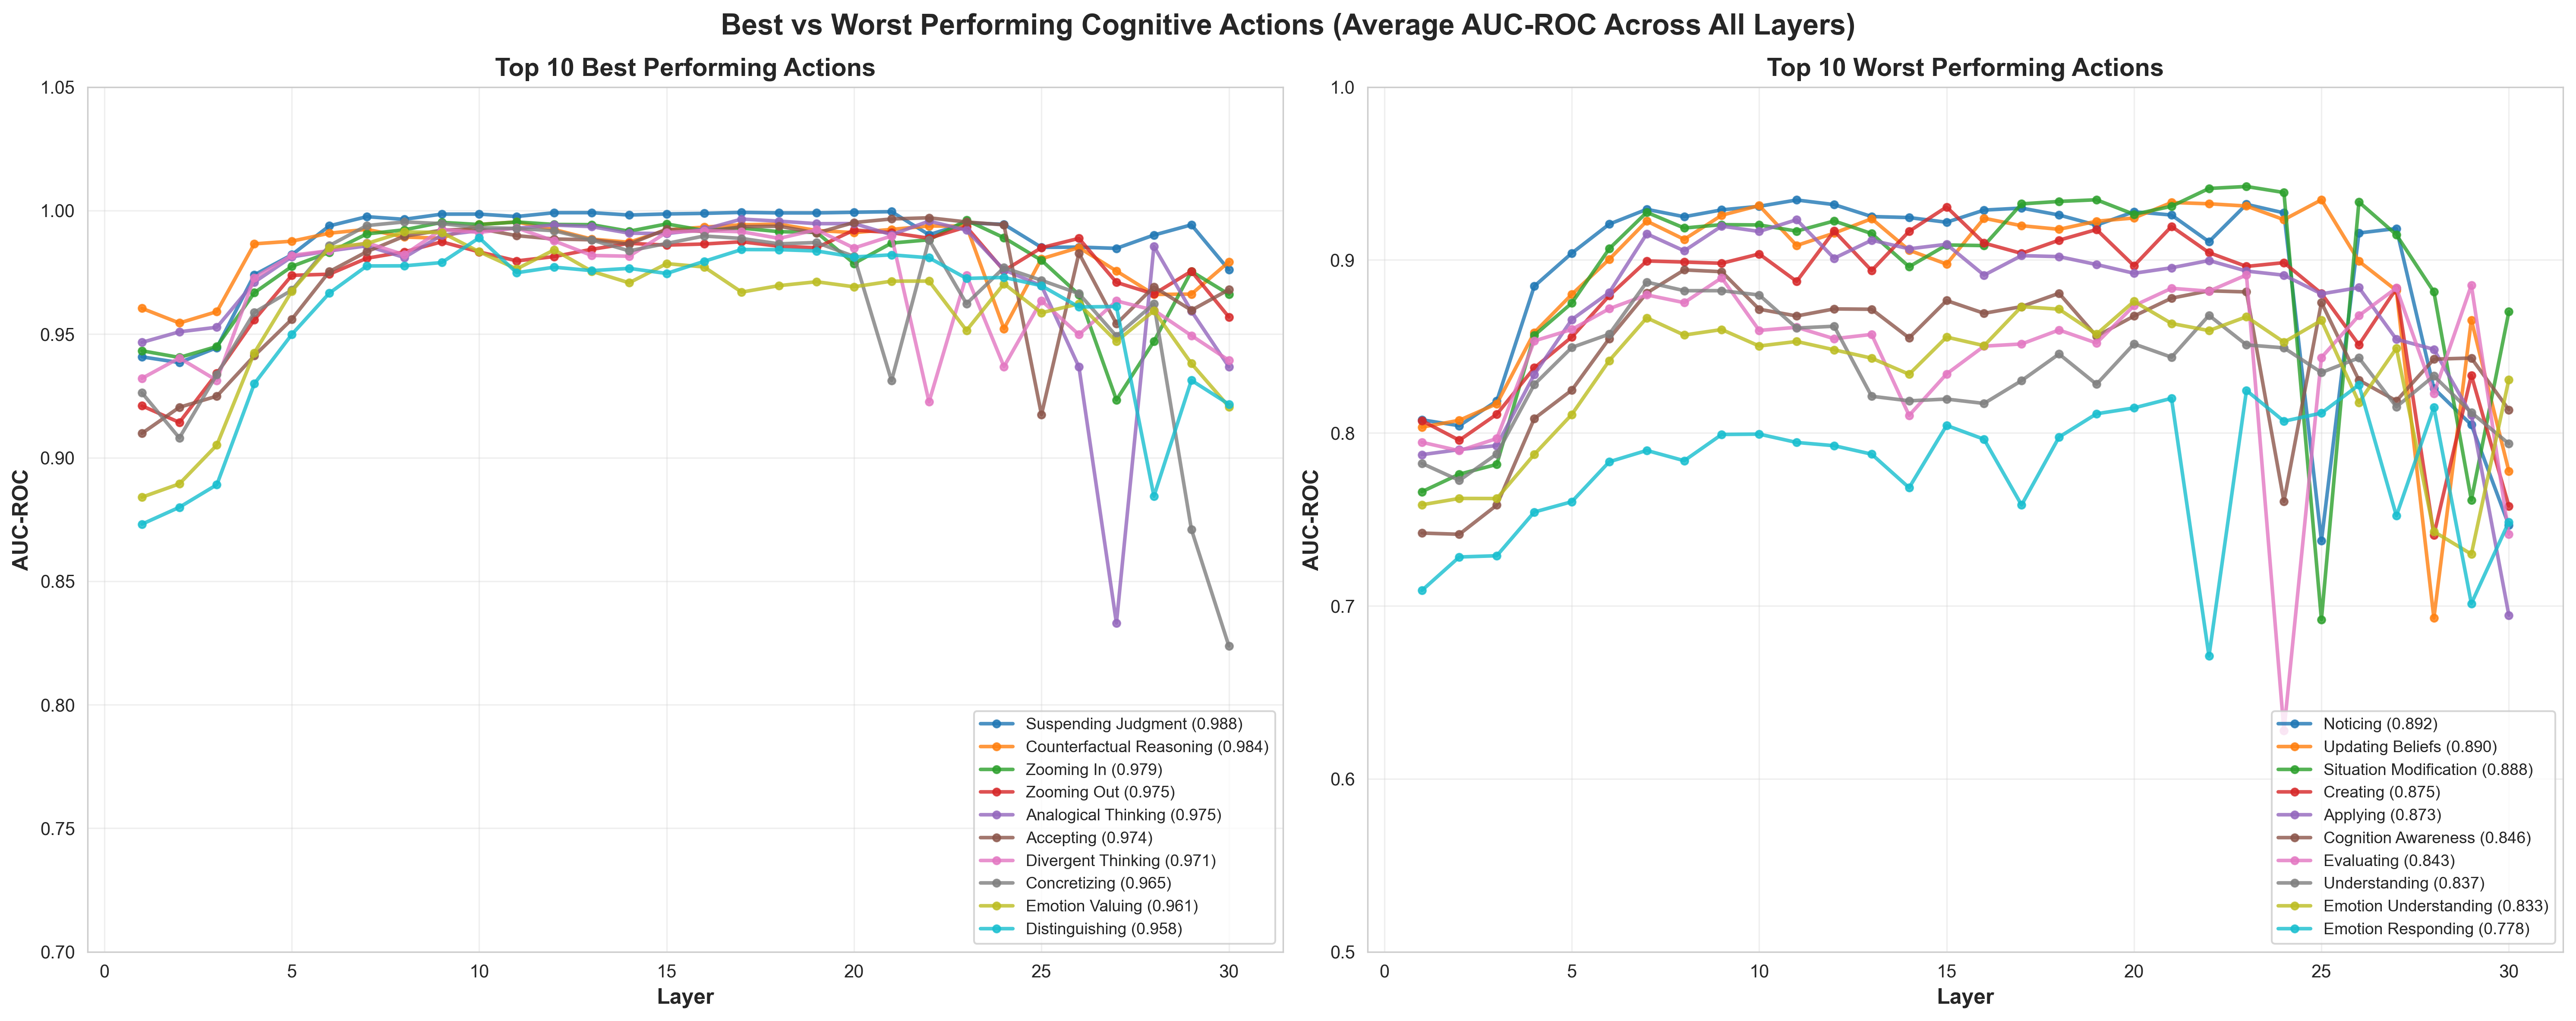
\includegraphics[width=\textwidth]{../data/best_worst_actions.png}
\caption{Comparison of top 10 and bottom 10 performing cognitive actions ranked by average AUC-ROC across all layers. Best performers like \textit{suspending\_judgment} (0.988) and \textit{counterfactual\_reasoning} (0.984) show consistently high performance and distinct activation patterns across most layers. Worst performers like \textit{emotion\_responding} (0.778) and \textit{understanding} (0.837) exhibit more variability and lower overall discrimination ability, suggesting these concepts may be more distributed or context-dependent in the model's representation space.}
\label{fig:best_worst}
\end{figure*}

\end{document}
